\documentclass[12pt, a4paper,oneside]{book}
\newcommand{\re}{\mathrm{e}}
\newcommand{\ri}{\mathrm{i}}
\newcommand{\rd}{\mathrm{d}}
\def\semicolon{\nobreak\mskip2mu\mathpunct{}\nonscript\mkern-\thinmuskip{;}
\mskip6muplus1mu\relax} % This defines the semicolon command

        % allows index generation
\usepackage{graphicx}        % standard LaTeX graphics tool
                             % when including figure files
\usepackage{multicol}        % used for the two-column index




\usepackage{color,tikz}
%\usepackage[unicode,bookmarks,bookmarksopen,bookmarksopenlevel=2,colorlinks,linkcolor=blue,citecolor=green]{hyperref}

\usepackage{amsmath,eucal,amssymb}
\usepackage{mathrsfs,graphicx,texdraw}
\usepackage{fancyhdr,framed}
\usepackage{tikz, tikz-3dplot}
\usepackage{tkz-euclide}
\usetikzlibrary{decorations.fractals}
\usetikzlibrary{decorations.footprints}




\usepackage{palatino}

\usepackage[latin1]{inputenc}

\usepackage[T1]{fontenc}
%\usepackage[dvips]{graphicx}
%\usepackage{times}


\definecolor{prempurple}{HTML}{37003c} % purple
\definecolor{premgreen}{HTML}{00ff87} % green
\definecolor{prempink}{HTML}{ff2882} % pink


\def\grole{\mathrel{\mathchoice {\vcenter{\offinterlineskip\halign{\hfil
$\displaystyle##$\hfil\cr>\cr\noalign{\vskip-1.5pt}<\cr}}}
{\vcenter{\offinterlineskip\halign{\hfil$\textstyle##$\hfil\cr
>\cr\noalign{\vskip-1.5pt}<\cr}}}
{\vcenter{\offinterlineskip\halign{\hfil$\scriptstyle##$\hfil\cr
>\cr\noalign{\vskip-1pt}<\cr}}}
{\vcenter{\offinterlineskip\halign{\hfil$\scriptscriptstyle##$\hfil\cr
>\cr\noalign{\vskip-0.5pt}<\cr}}}}}

\newenvironment{rcases}
  {\left.\begin{aligned}}
  {\end{aligned}\right\rbrace}

\newenvironment{lcases}
  {\left\lbrace\begin{aligned}}
  {\end{aligned}\right.}

\newtheorem{theorem}{Theorem}[section]
\newtheorem{lemma}[theorem]{Lemma}
\newtheorem{proposition}[theorem]{Proposition}
\newtheorem{corollary}[theorem]{Corollary}
\newtheorem{definition}[theorem]{Definition}
\newtheorem{example}[theorem]{Example}
\newtheorem{remark}[theorem]{Remark}

\newenvironment{proof}[1][Proof]{\begin{trivlist}
\item[\hskip \labelsep {\bfseries #1}]}{\end{trivlist}}
\newenvironment{solution}[1][Solution]{\begin{trivlist}
\item[\hskip \labelsep {\bfseries #1}]}{\end{trivlist}}

\newcommand{\qed}{\nobreak \ifvmode \relax \else
      \ifdim\lastskip<1.5em \hskip-\lastskip
      \hskip1.5em plus0em minus0.5em \fi \nobreak
      \vrule height0.75em width0.5em depth0.25em\fi}

\numberwithin{equation}{section}
\def\Ad{{\mbox{Ad}}}
\def\im{{\mbox{Im}}}
\def\Re{{\mbox{Re}\;}}
\def\ad{\mathrm{ad\,}}
\def\openone{\leavevmode\hbox{\small1\kern-3.3pt\normalsize1}}
\def\Res{\mathop{\mbox{Res}\,}\limits}
\def\biglb{\big[\hspace*{-.7mm}\big[}
\def\bigrb{\big]\hspace*{-.7mm}\big]}


\def\bigrbt{\mathop{\bigrb }\limits_{\widetilde{\;}}}
\def\biggrbt{\mathop{\biggrb }\limits_{\widetilde{\;}}}
\def\Bigrbt{\mathop{\Bigrb }\limits_{\widetilde{\;}}}
\def\Biggrbt{\mathop{\Biggrb }\limits_{\widetilde{\;}}}

\def\bPhi{\mathbf{\Phi}}
\def\bM{\mathbf{M}}
\def\bm{\mathbf{m}}
\def\bbbc{{\Bbb C}}
\def\bbbr{{\Bbb R}}
\def\bbbz{{\Bbb Z}}
\def\bbbs{{\Bbb S}}
\def\diag{\mbox{diag}\,}
\def\tr{\mbox{tr}\,}

\textwidth=17cm   \textheight=24.5cm \voffset=-2cm

\evensidemargin=-0.5cm \oddsidemargin=-0.5cm

 \renewcommand{\baselinestretch}{1.5}

%%%%%%%%fancy header%%%%%%%%%%%%%%%%%

\usepackage{fancyhdr}
\pagestyle{fancy}
\usepackage{calc}
\newlength{\pageoffset}
\setlength{\pageoffset}{0cm} % use whatever you like
\fancyheadoffset[LE,RO]{\pageoffset}
\renewcommand{\chaptermark}[1]{\markboth{#1}{}}
\renewcommand{\sectionmark}[1]{\markright{\thesection\ #1}}
\fancyhf{}
\fancyhead[LE]{\makebox[\pageoffset][l]{\thepage}\hfill\leftmark}
\fancyhead[RO]{\rightmark\hfill\makebox[\pageoffset][r]{\thepage}}
\fancypagestyle{plain}{%
    \fancyhead{} % get rid of headers
    \renewcommand{\headrulewidth}{0pt} % and the line
}

%%%%%%%%%%%%%%%%%%%%%%%%%%%%%%%%%%%%

\arraycolsep=2pt

%%%%Fancy Chapter%%%

%\usepackage{lmodern}
\usepackage{graphicx}
\usepackage{xcolor}
\usepackage{titlesec}
\usepackage{microtype}
\usepackage{lipsum}

\titleformat{\chapter}[display]
  {\normalfont\bfseries\color{prempurple}}
  {\filleft\hspace*{-60pt}%
    \rotatebox[origin=c]{90}{%
      \normalfont\color{prempurple}\Large%
        \textls[180]{\textsc{\chaptertitlename}}%
    }\hspace{10pt}%
    {\setlength\fboxsep{0pt}%
    \colorbox{prempurple}{\parbox[c][3cm][c]{2.5cm}{%
      \centering\color{premgreen}\fontsize{80}{90}\selectfont\thechapter}%
    }}%
  }
  {10pt}
  {\color{premgreen}\titlerule[2.5pt]\vskip3pt
  \titlerule\vskip10pt\color{prempurple}\LARGE\sffamily}

% hyperref should be loaded after all other packages
% aliascnt is needed to get \autoref (from hyperref) to work correctly with custom amsthm theorems
\usepackage{aliascnt}
\usepackage[colorlinks,linkcolor=prempink,citecolor=premgreen, linktoc=all]{hyperref}

% removes dots in table of contents
\makeatletter
\renewcommand\@dotsep{140}   % default value 4.5
\makeatother



\begin{document}


\thispagestyle{empty}

\begin{minipage}{0.2\textwidth}
\centerline{\includegraphics[width=.4\textwidth]{essex} }
\end{minipage}
\begin{minipage}{0.8\textwidth}

$ \qquad \qquad \qquad ${\LARGE \bf \sl University of Essex}

{\LARGE \bf Department of Mathematical Sciences}

\end{minipage}

\begin{center}

\noindent\textcolor{prempurple}{\rule{\linewidth}{4.8pt}}

\vspace{1cm}

{\LARGE \sc  MA838: Capstone Project}

\vspace{1.5cm}

{\Huge{A Data Analytics Approach to Fantasy Football Management}}

\vspace{1.5cm}

{\Large \bf Reece Lance}

\vspace{0.5cm}

{\Large \bf 1804752}

\vspace{1.5cm}

\centerline{\includegraphics[width=0.75\textwidth]{prem_logo.jpeg}}

\vspace{1.5cm}

{\Large {Supervisor:} {\bf Dr Andrew Harrison}}

\vspace{.25cm}

\noindent\textcolor{prempurple}{\rule{\linewidth}{4.8pt}}

\vspace{1cm}
{\Large \today }\\[4pt]
\end{center}
\newpage
\tableofcontents

\listoffigures
\listoftables


\chapter{Introduction}\label{ch:1}

You can start with some introduction of your project and background. 


You can make figures from files as you can see in Figure \ref{fig:A3.1}. For this you need to use include graphics. 

\begin{figure}[htb]
\centerline{\includegraphics[width=1\textwidth]{Figure}}
\caption{The Gauss map $\mathbf{g}_{K}$ takes $x\in \partial K$ to the outer normal $n_x\in\mathbb{S}^{n-1}$ at that point}
\label{fig:A3.1}
\end{figure}


While writing be clear and precise and give references whenever necessary. You may like to use theorem, definition, lemma, and example environments provided by \LaTeX. For example,

Pioneering work of Emmy Noether \cite{Noether} provides a connection between symmetries and conservation laws. This result, known as Noether's theorem states that

\begin{theorem}[Noether, \cite{Noether}]
Every differentiable symmetry of the action of a physical system has a corresponding conservation law.
\end{theorem}

\begin{example}
This is an example.
\end{example}

\begin{lemma}
This is a lemma.
\end{lemma}

\begin{definition}
In 1950, Alan Turing published an article \cite{Turing} in \textit{Mind} 
titled ``Computing Machinery and Intelligence'' where he considered the question ``Can machines think?''. This is known as {\bf Turing's Test}. 
\end{definition}

\begin{remark}
This is a very important remark. 
\end{remark}

You can also make figures using \LaTeX packages for figures (e.g. the {\tt TikZ package}) as you can see in Figure \ref{fig:tikz}.

\begin{figure}[htb]
\begin{center}
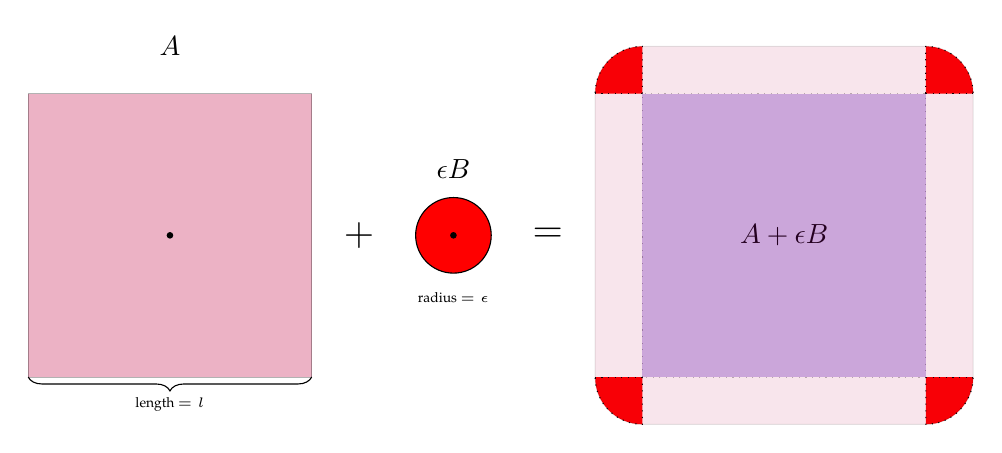
\begin{tikzpicture}[scale=.6]
\draw[fill=purple, opacity=.3] (-3,-3) rectangle (3,3);
\fill (0,0) circle [radius=2pt];
\node at (0,4) {$A$};
\node at (4,0) {\Large $+$};
\draw[fill=red] (6,0) circle (.8cm);
\fill (6,0) circle [radius=2pt];
\node[above] at (6,1) {$\epsilon B$}; 
\node[below] at (6,-1) {\tiny radius $=\epsilon$};
\node at (8,0) {\Large $=$};

\draw [decorate,decoration={brace,amplitude=5pt, mirror}]
(-3,-3) -- (3,-3) node[below] [black,midway, yshift=-4pt] {\tiny length $=l$};

\draw[dotted, fill=blue, opacity=.1] (10,-3) rectangle (16,3);

\node at (13,0) {$A +  \epsilon B$};


\draw[dotted, fill=blue, opacity=.1] (10,-3) rectangle (16,3);

\draw[dotted, fill=red] (10,-3)--(10,-4) arc (270:180:1);
\draw[dotted, fill=red] (10,3)--(10,4) arc (90:180:1);
\draw[dotted, fill=red] (16,3)--(16,4) arc (90:0:1);
\draw[dotted, fill=red] (16,-3)--(16,-4) arc (270:360:1);

\draw[dotted] (10,-3)--(9,-3);
\draw[dotted] (16,-3)--(17,-3);

\draw[dotted] (16,3)--(16,4);
\draw[dotted] (16,3)--(17,3);

\draw[dotted] (10,3)--(9,3);


\draw[dotted, fill=purple, opacity=.1] (10,-3) rectangle (16,3);
\draw[fill=purple, opacity=.1] (16,4)--(10,4) arc (90:180:1)--(9,-3)--(9,-3) arc (180:270:1)--(10,-4)--(16,-4)--(16,-4) arc (270:360:1)--(17,-3)--(17,3) arc (0:90:1);
\end{tikzpicture}
\end{center}
\caption{Minkowski sum of a square and ball with radius $\epsilon$}
\label{fig:tikz}
\end{figure}


\chapter{Data Preprocessing}\label{ch:2}

Preprocessing is a vital process when working with raw data, in order to have the data in an
understandable form to extract and use meaningful information. This process involves
amending the data to the point where there is no incomplete, inconsistent or outlying values
which could cause errors when applying a model. Typically, most sets of data will have at
least one of these issues; this dataset is no different.

\section{Retrieving the data from the API}\label{sec:2.1}

... goes here.

\section{Analysing the data}\label{sec:2.2}

... goes here.

\chapter{Your second main chapter}\label{ch:3}

The text goes here ... 

\section{Your first section of the second main chapter}\label{sec:3.1}

... goes here.

\section{Your second section of the second main chapter}\label{sec:3.2}

... goes here.

\chapter{Conclusions}\label{ch:concl}
And here is the final chapter showing how clever you are ....




% Comment the following THREE lines if you do NOT have an Appendix
\appendix
\chapter{A Long Proof}

Text goes here

% If you need more than one appendix, then just use another \chapter command
%\chapter{Yet Another Appendix}

\chapter{Another Appendix}

Text goes here




\begin{thebibliography}{999}

%%% Bibliography items should be below this here %%%



\bibitem{Frenzel}
Timothy, Frenzel.
\newblock `Fantasy Premier League API Endpoints: A Detailed Guide'.
\newblock {\em Medium, 8 October 2020, https://medium.com/@frenzelts/fantasy-premier-league-api-endpoints-a-detailed-guide-acbd5598eb19.}



\end{thebibliography}






\end{document}

